\documentclass[border=0cm]{standalone}
%\documentclass{article}
\usepackage{tikz}
\usepackage[width=0.5,tiewidth=0.7]{strands}

\begin{document}
%https://latexdraw.com/draw-a-sphere-in-latex-using-tikz/
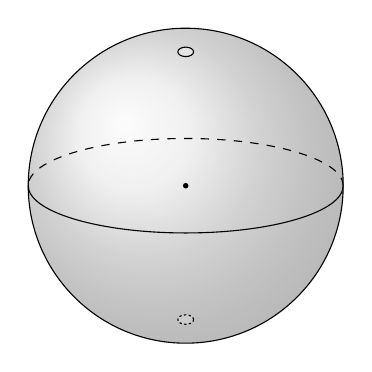
\begin{tikzpicture}
\def\a{3mm}
\shade[ball color = gray!40, opacity = 0.4] (0,0) circle (2cm);
\draw (0,0) circle (2cm);
\draw (-2,0) arc (180:360:2 and 0.6);
\draw[dashed] (2,0) arc (0:180:2 and 0.6);
\fill[fill=black] (0,0) circle (1pt);
\draw [fill=white!80!gray] (0,0.85 * 2) ellipse (1mm and 0.6mm);
\draw [fill=white!60!gray,dash pattern={on 0.3mm off 0.3mm}] (0,-0.85 * 2) ellipse (1mm and 0.6mm);
\end{tikzpicture}
\end{document}